\documentclass{beamer}
\usepackage[utf8x]{inputenc}
\usepackage[english,russian]{babel}
\usepackage[section]{placeins}
\usepackage{upgreek}
\usepackage{graphicx}
% \usepackage[left=3cm, right=1.5cm, top=2cm, bottom=2cm]{geometry}
\usepackage{caption}
\usepackage{subcaption}
\usepackage{indentfirst}
% \usepackage{wrapfig}
\usepackage{amsmath}
\usepackage{gensymb}
% \usepackage{setspace}
% \usepackage{placeins}
\graphicspath{{images/}}

% \textheight 24.5cm % 29.7-2-2=25.7
% \textwidth 17cm % 21-2.5-1.5=17.0
% \hoffset -0.04cm %2.5-2.54=-0.04 слева 3см
% \voffset -0.54cm %2-2.54=0.54 сверху 2см
% \oddsidemargin 0cm
% \headheight 0cm
% \headsep 0cm
% \topmargin 0cm
% \onehalfspacing

% \textheight 25.7cm % 29.7-2-2=25.7
% \textwidth 17cm % 21-2.5-1.5=17.0
% \hoffset -0.04cm %2.5-2.54=-0.04 слева 3см
% \voffset -1.04cm %2-2.54=0.54 сверху 2см
% \oddsidemargin 0cm
% \headheight 0cm
% \headsep 0cm
% \topmargin 0cm
% \setcounter{page}{1}
\def\sigspace{\\[1em]
\underline{\hspace{5cm}}\\[-0.2em]}

\def\etal{{et~al.}}
\usetheme{Madrid}
\usecolortheme{beaver}
% \setbeamercolor{navigation symbols}{fg=red}
\setbeamercolor{palette sidebar secondary}{fg=black}
\setbeamercolor{section in sidebar shaded}{fg=gray}
\usefonttheme[onlymath]{serif}
\setbeamertemplate{bibliography item}{\insertbiblabel}
\setbeamercolor*{bibliography entry title}{fg=black}
\setbeamercolor*{bibliography entry author}{fg=black}
\setbeamercolor*{bibliography entry location}{fg=black}
\setbeamercolor*{bibliography entry note}{fg=black}

\setbeamertemplate{caption}[numbered]


\begin{document}

\title[]{Образование эмиссионных линий в магнитосферах молодых звезд}
\author[]{\textbf{Д.~В.~Дмитриев\inst{1}, В.~П.~Гринин\inst{1,2}, Н.~А.~Катышева\inst{3}}}
\institute[ГАОРАН, СПбГУ, ГАИШ]{\inst{1} Главная (Пулковская) Астрономическя Обсерватория РАН, Санкт-Петербург, Россия \\
  \inst{2} Санкт-Петербургский Государственный Университет, Санкт-Петербург, Россия \\
  \inst{3} Государсвенный Астрономический Институт им. П.~К.~Штернберга при МГУ~им.~Ломоносова, Москва, Россия \\ ~\\
  \small{Звезды, планеты и их магнитные поля}}
\date{2018 год}

\frame[noframenumbering]{\titlepage}
%\frame[noframenumbering]{Здравствуйте. Моя дипломная работа называется ... .} 

\section{Введение}
\begin{frame}


\frametitle{Введение}
Работа посвящена разработке модели аккреции водородного газа на звезды типа Т Тельца
\begin{itemize}
\item Молодые звезды, PMS
\item Медленная скорость вращения $\approx 15 \text{км/с}$
\item Масса от 0.2 до 2 $\text{M}_\odot$
\item T$_\text{eff} \approx $ 4000 К  
\item Магнитное поле 1-2 кГс
\end{itemize}
Наблюдения и теория показывают, что сильное магнитное поле может захватывать аккрецирующий газ, в результате чего образуется магнитосфера.
\end{frame}

%\frame[noframenumbering]{Она посвящена разработке модели аккреции водородного газа на звезды типа Т Тельца. Это медленно вращающиеся , со скоростью около 15 км/с на экваторе, молодые звезды, еще не достигшие главной последовательности, часто окруженные протопланетными дисками. Они имеют массу от нескольких десятых до 2-3 масс Солнца и эффективую температуру в среднем 4000 кельвинов. Также они имеют сильное магнитное поле в районе 1-2 кГс. Наблюдения и теория показывают, что сильное магнитное поле способно захватывать аккрецирующий из диска газ, в результате чего образуеся магнитосфера. В ней образуются различные эмиссионные линии.}

% \begin{frame}
% При взаимодействии газа с магнитным полем звезды лишний угловой момент уносится дисковыми ветрами.
% \begin{figure}
% \centering
% 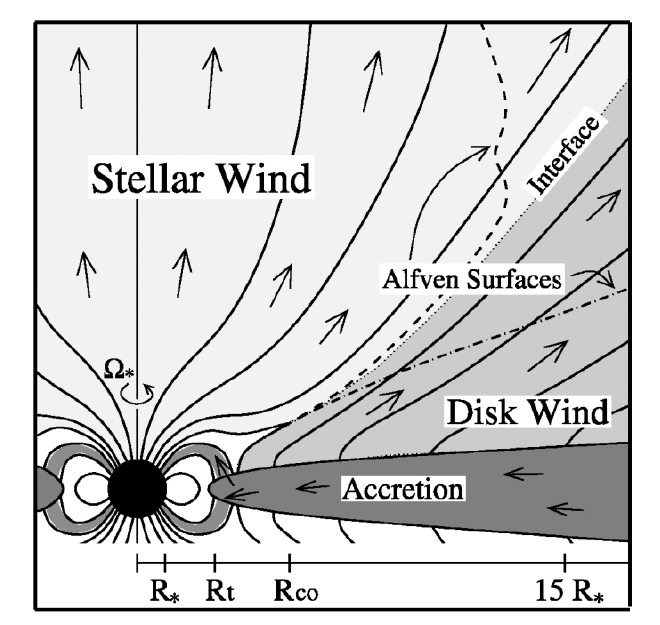
\includegraphics[width=0.6\textwidth]{mag.png}
% \caption{ \footnotesize из Matt, S., Pudritz, R.E., ApJL, 2005, 632, L135}
% \end{figure}

% \end{frame}

\subsection{Наблюдаемые профили линий}

\begin{frame} 
\frametitle{Наблюдаемые профили линий}

\begin{figure}[h] 
\centering
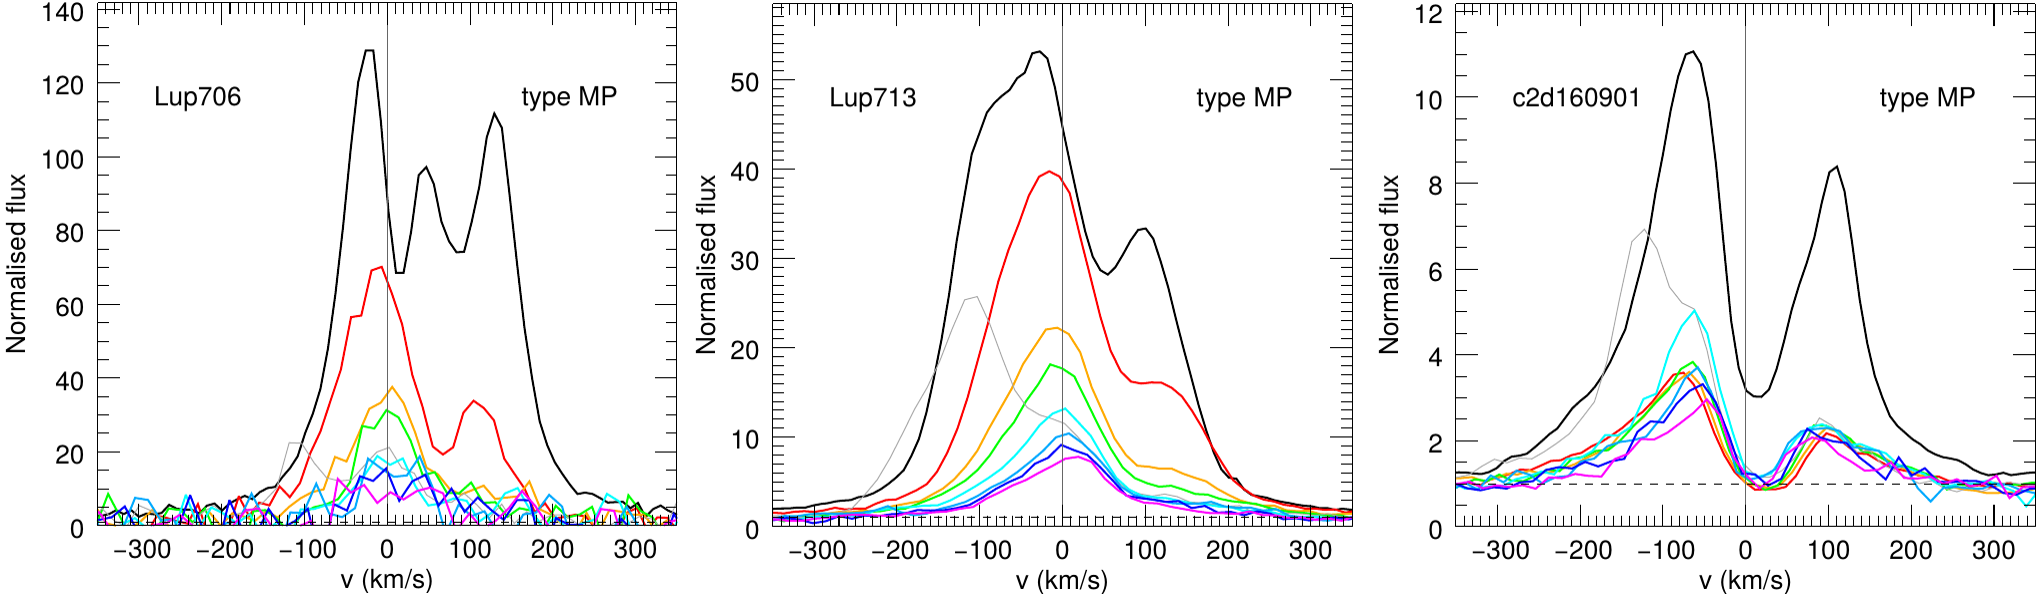
\includegraphics[width=\textwidth]{profiles.png}
\caption{ Наблюдаемые профили линий бальмеровской серии, Antoniucci \etal\ (2017)}
\label{fig:profiles}
\end{figure}

% Цель работы --- создать инструмент, способный воспроизводить наблюдаемые профили.

\end{frame}

%\frame[noframenumbering]{На этом слайде показаны профили линий бальмеровской серии, наблюдающиеся в спектрах звезд типа Т Тельца. профили имеют характерные признаки аккреции, такие как ассиметрия, меньшая интенсивность, с красной стороны. Цель моей работы --- создать инструмент, способный воспроизводить наблюдаемые профили. Работа актуальна, так как моделирование профилей позволяет оценивать параметры звезд и аккрецирующего газа, темп аккреции, тем самым проверяя теорию.}

\begin{frame}
\frametitle{Переменность профилей линий}
\begin{figure}[h]
\centering
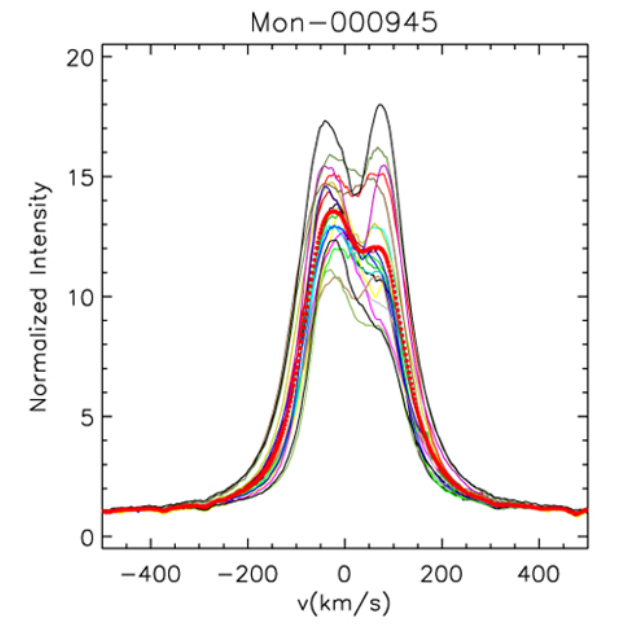
\includegraphics[width=0.5\textwidth]{profilevar.png}
\caption{Переменность линии H$\alpha$, Sousa \etal\ (2016)}
\end{figure} 
\end{frame}

%\frame[noframenumbering]{В спектрах звезд типа Т Тельца также часто наблюдается вращательная модуляция профилей линий. Ее часто связывают с отклонением оси магнитного пол яот оси вращения. В работе также моделируется такая переменность.}


\subsubsection{Основные излучающие области звезд типа Т Тельца}
\begin{frame}
\frametitle{Основные излучающие области звезд типа Т Тельца}
\begin{columns}[T]
\begin{column}{0.5\textwidth}
\begin{figure}
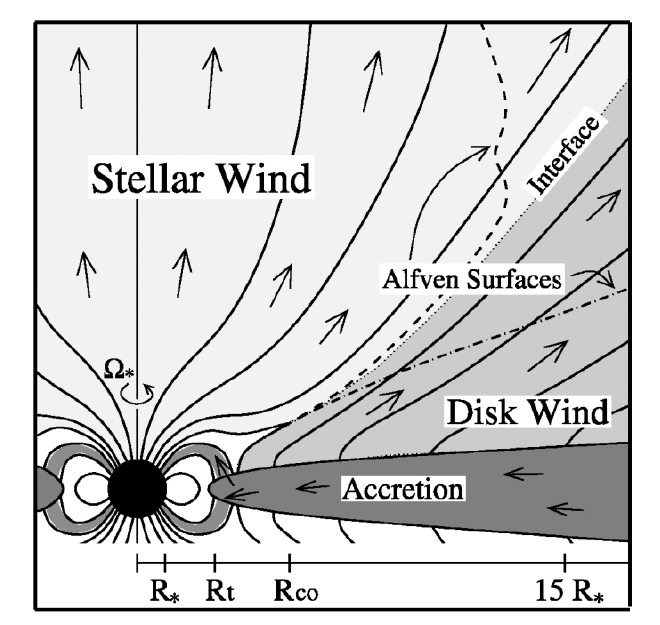
\includegraphics[width=\textwidth]{mag.png}
\end{figure}
\end{column}
\begin{column}{0.5\textwidth}
\begin{itemize}
\item Магнитосфера (Hartmann \etal\ 1994, Muzerolle \etal\ 2001)
\item Дисковый и магнитосферные ветра (Kurosawa \etal\ 2006, Lima \etal\ 2010, Petrov \etal\ 2014)
\item Горячее аккреционное пятно (Lamzin 1998, Dodin 2018)
\end{itemize}
\end{column}
\end{columns}
\end{frame}

%\frame[noframenumbering]{В спектр и профили линий у звезд т тельца помимо магнитосферы ыносят заметный вклад также и другие области. Например дичковый и магнитосферные ветра, а также горячее паккреционное пятно. Для полного моделирования профилей линий необходимо учитывать все эти составляющие. В нашей лаборатории мы уже имеем инструменты для рассчетов ветровых компонентов. Сейчас мы разработали инструмент, позволяющий моделировать магнитосферу.}

\section{Модель магнитосферы}

\begin{frame}
\frametitle{Модель магнитосферы}
\begin{columns}[T]
\begin{column}{0.5\textwidth}
\begin{figure}
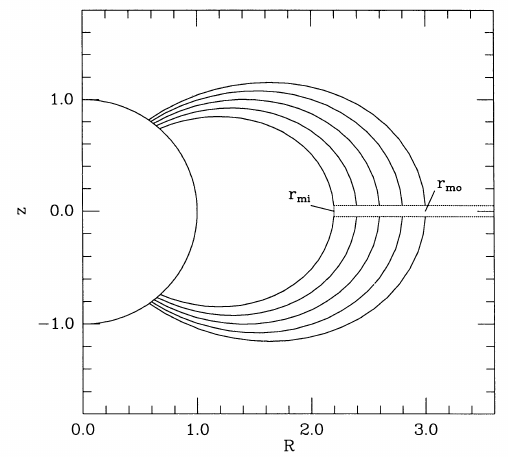
\includegraphics[width=\textwidth]{hartgrid.png}
\end{figure}
\end{column}
\begin{column}{0.5\textwidth}
\begin{itemize}
\item Дипольная магнитное поле
\begin{equation} \label{eq:dipole}
r = r_\text{m} \sin^2 \theta \nonumber
\end{equation}
\item Вмороженность газа, границы магнитосферы 
\begin{equation}
r_\text{mi} \le r_\text{m} \le r_\text{mo} \nonumber
\end{equation}
\item Твердотельное вращение
\item Плотность и температура из работы Хартманна и др. (1994)
\end{itemize}
\end{column}
\end{columns}
\end{frame}

%\frame[noframenumbering]{На рисунке схематично показана модель магнитосферы, использующаяся в работе. Мы предполагаем дипольное магнитное поле, в котором невязко движется полностью вмороженный в него газ от диска к звезде. Магнитосфера имеет границы --- rmi rmo. Мы во многом следуем работе Хартманна и др. 1994 года, и из нее берем зависимости плотности и температуры в магнитосфере.}

\begin{frame}
\begin{itemize}
\item Дополнительный нагрев у поверхности звезды, Додин (2018)
\begin{equation} \label{eq:temp}
 T = T_{\text{hart}} + T_\text{hot}\exp\left(-\frac{r - R_\star}{d_\text{hot} R_\star}\right)
\end{equation}
\item Водородный газ
\item Метод Соболева с учетом нелокального радиационного взаимодействия 
\end{itemize}

\end{frame}

%\frame[noframenumbering]{При этом мы вносим дополнительный нагрев в магнитосферу у поверхности звезды, связвнный с аккреционным пятном. В этом году Додин показал, что температура в аккреционом пятне может достишать 10-20 тысяч градусов, и пятно может нагревать ближайшие слои магнитосферы. Поэтому мы добавляем к температуре экспоненциально затухающий от поверхности звезды член. Для расчета переноса излучения в водородном газе мы используем приближение соболева с учетом нелокального радиационного взаимодействия.}

% \subsection{Уравнения ст}

\begin{frame}
\frametitle{Система уравнений стационарности}
% \verysmall
\begin{align}
n_i & \Bigg[ \sum\limits_{j=1}^{i-1} (A_{ij} + B_{ij}J_{ij}) + \sum\limits_{k=i+1}^\infty B_{ik}J_{ik} + \nonumber \\
 +\ &n_e  ( q_{ic} + \sum\limits_{j \neq i}^\infty q_{ij} ) + B_{ic}WJ_{ic}^\star \Bigg] = \nonumber \\
 =\ & \sum\limits_{k=i+1}^\infty n_k (A_{ki} + B_{ki}J_{ki}) + \sum\limits_{j=1}^{i-1} n_jB_{ji}J_{ij} + \nonumber \\
 +\ & n_e \sum\limits_{j\neq i}^\infty n_jq_{ji} + n_en^+C_i + n_e^2n^+Q_{ci} \\
 & i=1,\ 2,\ ... \nonumber
\end{align}
\normalsize
\footnotesize Катышева, Н.А., Гринин, В.П., Изв. КрАО, 1980, 62, 52
\end{frame}

%\frame[noframenumbering]{На этом слайде показана система уравнений стационарности, которая решалась в работе для определения состояния водородного газа. Формально система имеет бесконечное число уравнений, однако бесконечные суммы обрезаются на 15 уровне, так как учет более высоких уровней не имеет смысла для данной задачи.} 

\subsection[Нелокальное взаимодействие]{Учет нелокального радиационного взаимоействия}

% \subsubsection[Нелокальное взаимоействие]{Учет нелокального радиационного взаимоействия}
\begin{frame}
\frametitle{Учет нелокального радиационного взаимодействия}
Грачев, Гринин (1975)	, Rybicki, Hummer (1978) 
\begin{equation} 
J_{ki} = (1-\beta_{ik}(\vec{r}))S_{ki}(\vec{r}) + \beta_{ik}^\star(\vec{r})I^\star_{ki} + F_{ki}(\vec{r}), 
\end{equation}
\begin{equation} \label{eq:beta} \nonumber
\beta_{ik}(\vec{r}) = \frac{1}{4\pi}\int\limits_{(4\pi)} d\Omega(\vec{n})\frac{1-e^{\tau_{ik}(\vec{r},\vec{n})}}{\tau_{ik}(\vec{r},\vec{n})}, 
\end{equation}
\begin{equation} \label{eq:starbeta} \nonumber
\beta_{ik}^\star(\vec{r}) = \frac{1}{4\pi}\int\limits_{\Omega_\star} d\Omega(\vec{n})\frac{1-e^{\tau_{ik}(\vec{r},\vec{n})}}{\tau(\vec{r},\vec{n})}e^{-\sum_{j=1}^N\tau_{ik}(\vec{r_j},\vec{n})},
\end{equation}
\begin{equation} \label{eq:CPF} \nonumber
F_{ki}(\vec{r}) = \frac{1}{4\pi}\int\limits_{(4\pi)} d\Omega(\vec{n})\frac{1-e^{\tau_{ik}(\vec{r},\vec{n})}}{\tau(\vec{r},\vec{n})}\sum\limits_{j=1}^N S_{ki}(\vec{r_j}) (1-e^{\tau_{ik}(\vec{r_j},\vec{n})}) e^{-\sum_{e=1}^{j-1}\tau_{ik}(\vec{r_e},\vec{n})}
\end{equation}
\end{frame}

\begin{frame}
\frametitle{Учет нелокального радиационного взаимодействия}
\begin{figure}[h]
\centering
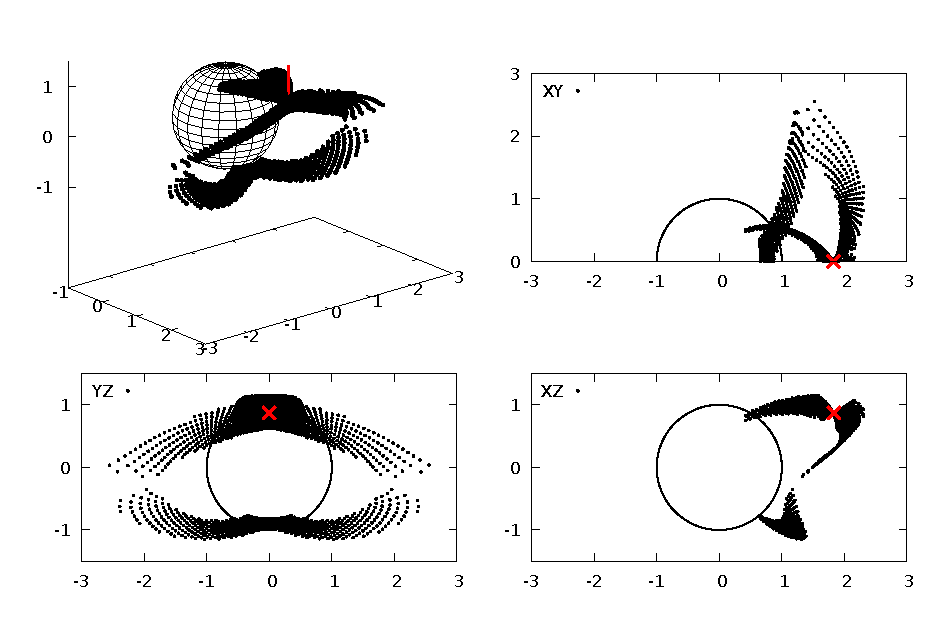
\includegraphics[width=0.9\textwidth]{surf.eps}
\end{figure}
% \end{figure}

\end{frame}

\begin{frame}
\frametitle{Учет нелокального радиационного взаимодействия}
\begin{figure}
\centering
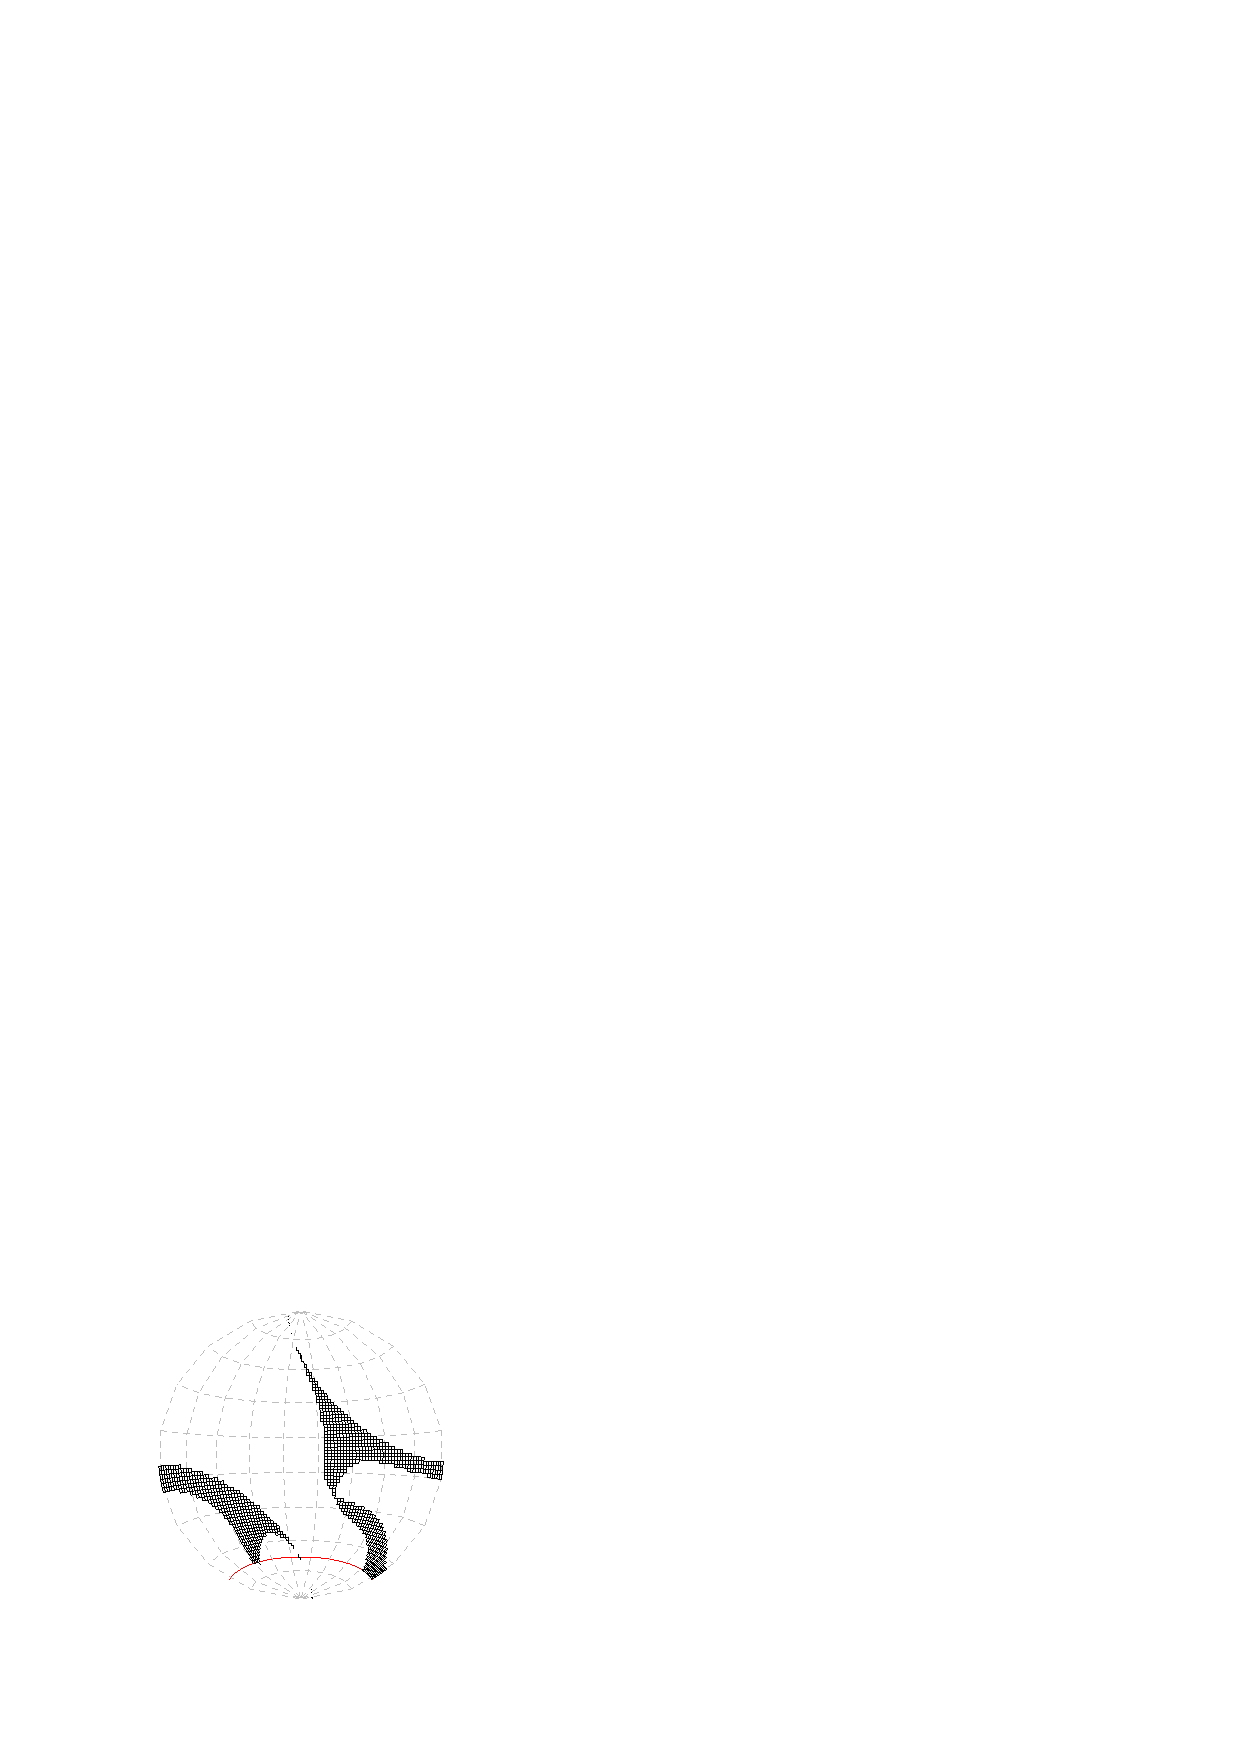
\includegraphics[width=0.5\textwidth]{sphere.pdf}
% \caption{Черным показаны направления, в которых можно встретить точку CP-поверхности, если начинать от порождающей ее точки (направления, в которых подынтегральное выражение в \eqref{eq:CPF} не обнуляется). Направление вниз --- направление на центр звезды, направление вверх --- от звезды. Показано только одно полушарие, так как поверхность симметрична относительно плоскости, в которой лежат ось симметрии и точка, ее порождающая. Красной кривой ограничена часть направлений, занимаемая звездой.}
% \label{fig:CPmap}
\end{figure}
\end{frame}


%\frame[noframenumbering]{Для решения системы необходимо знать среднюю интенсивность в линии. В приближении соболева она записывается вот так, так как из-за градиента скорости среда просветляется, и кванты могут поглощаться только в локальной области. Первый член в этом уравнении учитывает локальное взаимодействие. Второй член учитывает внешний источник излучения -- звезду, излучение которой мы считаем чернотельным. В некоторых случаях необходимо вносить еще один член, для учета нелокального радиоционного взаимодействия. Оно возникает из-за того, что некоторые области магнитосферы имеют нулевую лучевую скорость относительно друг-друга, и квант излученный в одной из них может поглотится в другой, тем самым перенося состояния возбуждения. Форма поверхности, которая взаимодействует таким образом с точкой в магнитосфере, показаной красным, поазана здесь. Также показаны проекции этой поверхности на координатные плоскости. Эффект нелокального взаимодействия сказывается больше всего в холодных частях магнитосферы, которые могут таким образом взаимодейстововать с горячими частями магнитосферы.}

\section{Расчет профиля линии}

\begin{frame}
\frametitle{Профиль коэффициента поглощения}
Для большинства линий использовался доплеровский профиль коэффициента поглощения
\begin{equation} \label{eq:profabsprof}
\alpha(\nu, z) = \frac{1}{\sqrt{\pi} \Delta\nu_D} \exp\left( -\left[ \frac{\nu - \nu_0}{\Delta\nu_D} - \frac{v_z(z)}{v_t}\right]^2\right)
\end{equation}
Для линии H$\alpha$ --- фойгтовский

\begin{equation} \label{eq:profabsfoigt}
\alpha(\nu, z) = \frac{1}{\sqrt{\pi} \Delta\nu_D}\ H\left(\frac{\delta}{\Delta\lambda_D},\ \left[ \frac{\nu - \nu_0}{\Delta\nu_D} - \frac{v_z(z)}{v_t}\right]\right)
\end{equation}

\small
\begin{align} \label{eq:foigtcoef}
\delta = 6.5\cdot 10^{-4} \ \mathring{\text{A}}\ +\ 4.4\cdot 10^{-4}\ \mathring{\text{A}} \ \frac{n_{\text{HI}}}{10^{16}\ \text{cm}^{-3}}\left(\frac{T}{5000 \text{K}}\right)^{0.3} + \nonumber \\ 
  +\ 1.174\cdot 10^{-3}\ \mathring{\text{A}}\ \frac{n_e}{10^{12}\ \text{cm}^{-3}}\ + \ 8.98\cdot 10^{-4}\ \mathring{\text{A}}\ \frac{n_\text{HI}}{10^{16}\ \text{cm}^{-3}} 
\end{align}
\normalsize
\end{frame}

%\frame[noframenumbering]{Для расчета интенсивности в линиях мы использовали доплеровский профиль поглощения, однако для линии На мы применяли фойгтовский профиль, так как в ней сильно сказываются лоренцовские крылья.}

\section{Результаты}
\subsection{Параметы модели}
\begin{frame}
\frametitle{Параметры модели}
\begin{table}[hb]
\centering
\small
\begin{tabular}[c]{|l r|}
	% \hline
	\multicolumn{2}{c}{\textbf{Параметры магнитосферы}} \\
	\hline
	$r_\text{mi}$ & $2.2 \text{R}_\star$\\
	\hline
	$r_\text{mo}$ & $3.0 \text{R}_\star$\\
	\hline
	$\dot{M}$  & от $10^{-9}$ до $10^{-7}$ M$_{\odot}$/год \\
	\hline
	$T_\text{max}$ & от 7500 до 8500 K  \\
	\hline
	$T_\text{hot}$ & 0, 3000, 5000 K  \\
	\hline
	$d_\text{hot}$ & 0.1 R$_\star$ \\
	\hline
	\multicolumn{2}{c}{\textbf{Параметры звезды}} \\
	\hline
	$R_\star $  & $2 R_\odot$ \\
	\hline
	$M_\star $ & $0.8 M_\odot$ \\
	\hline
	$T_\star $ & $4000\text{K} $ \\
	\hline
	$v_\text{eq}$ & 0, 15 км/с \\
	\hline
	\multicolumn{2}{c}{\textbf{Параметры ориентации оси магнитосферы}} \\
	\hline
	$i$ & от 15\degree до 75\degree \\
	\hline
	$\alpha$ & 0\degree, 15\degree \\
	\hline
	$\psi$ & от 0\degree до 180\degree \\
	\hline
\end{tabular}
\end{table}
\end{frame}

%\frame[noframenumbering]{в таблице перечисленны параметры магнитосферы со значениями, которые они принимали в работе. (перечисляю параметры)}

\subsection{Состояние газа в магнитосфере}

\begin{frame}
\frametitle{Температура}
\begin{figure}[!h]
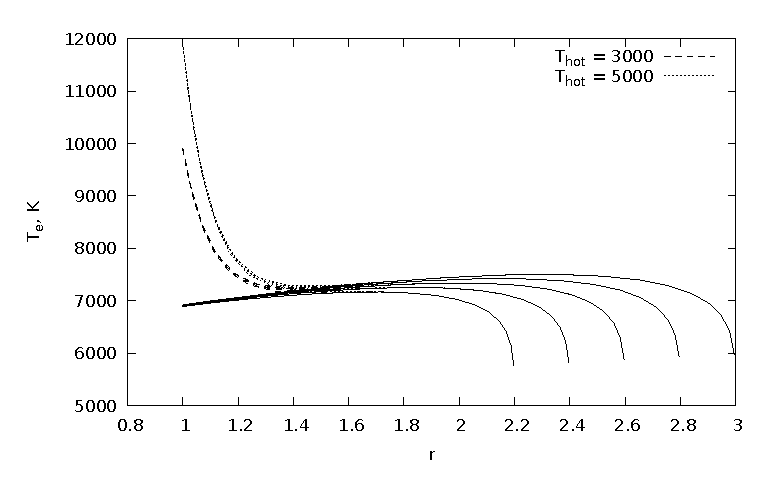
\includegraphics[width=\textwidth]{T_e.eps}
\end{figure}
\end{frame}

%\frame[noframenumbering]{На этом слайде показана зависимость температуры в магнитосфере от расстояния до звезды в ее радиусах. Темп аккреции 10^-7. Максимальная температура 7500 К. Показано влияние дополнительного нагрева с температурой 5 и 3 тысячи кельвинов и размером в 0.1 радиус звезды.} 

\begin{frame}
\frametitle{Электронная концентрация}
\begin{figure}[!h]
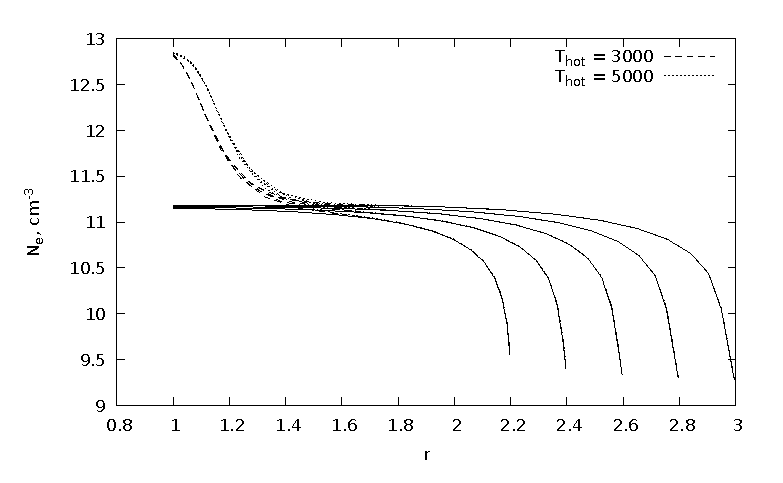
\includegraphics[width=\textwidth]{N_e.eps}
\end{figure}
\end{frame}

%\frame[noframenumbering]{Электронная концентрация для той же модели. Засчет дополнительного нагрева происходит быстрая ионизация у поверхности звезды.}

\begin{frame}
\frametitle{Населенность первого уровня}
\begin{figure}[!h]
\centering
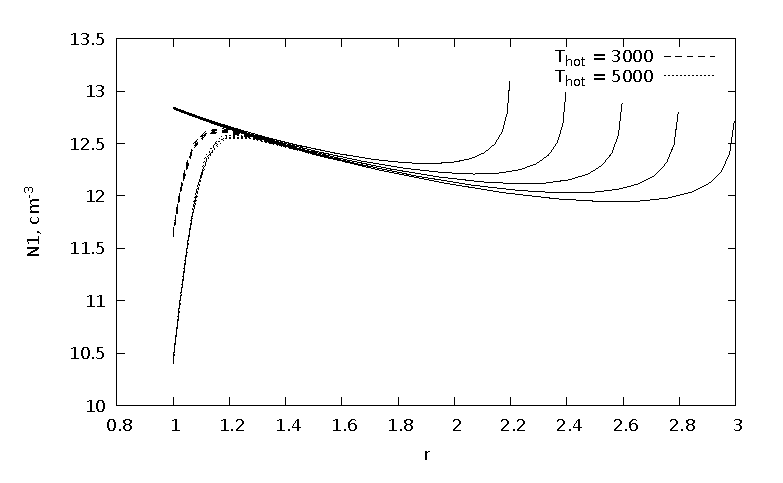
\includegraphics[width=\textwidth]{N1.eps}
\end{figure}
\end{frame}

%\frame[noframenumbering]{Населенность первого уровня, быстрая ионизация.}

\begin{frame}
\frametitle{Населенность второго уровня}
\begin{figure}[!h]
\centering
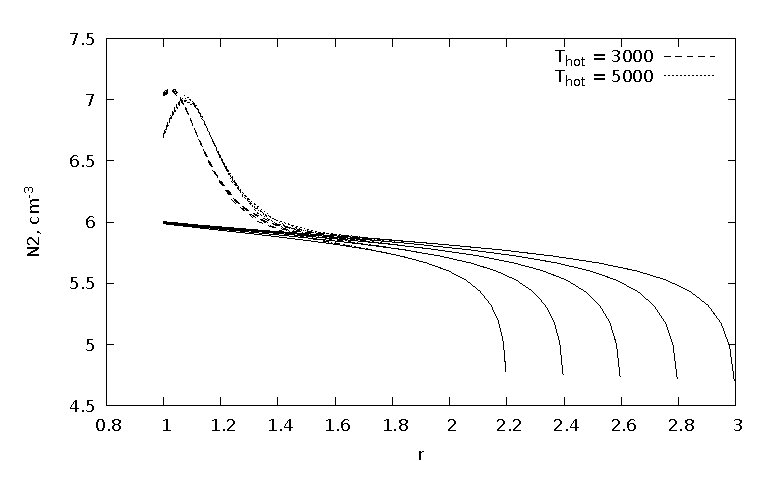
\includegraphics[width=\textwidth]{N2.eps}
\end{figure}
\end{frame}

%\frame[noframenumbering]{Населенность второго уровня, экстремум связан с тем, что ионизация сначала происходит через второй уровень, а затем уже напрямую с первого.}

\subsection[Профили линий]{Профили водородных линий без учета вращения магнитосферы}

\begin{frame}
\frametitle{Профили водородных линий. H$\alpha$}
\begin{figure}[h]
\centering
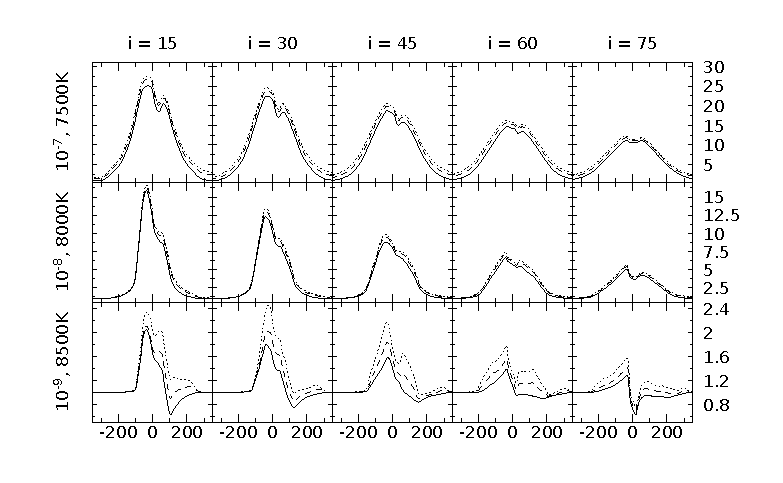
\includegraphics[width=\textwidth]{hot_5_Ha.eps}
\end{figure}
\end{frame}

%\frame[noframenumbering]{На этом слайде показаны профили линии На для различных моделей без учета вращения магнитосферы. Сверху написан угол наклона оси магнитосферы к лучу зрения. Слева --- темп аккреции и температура. Пунктиром и штрихом показан вклад дополнительного нагрева на 5 и 3 тысячи кельвинов. Видно, что для больших темпов аккреции линия сильно размыта из-за Лоренцовских крыльев. В целом линии уменьшают интенсивность и расширяются при увеличении угла наклона. Вклад нагрева сильновлияет только на профили с малым темпом аккреции.}  

\begin{frame}
\frametitle{Профили водородных линий. H$\beta$}
\begin{figure}[h]
\centering
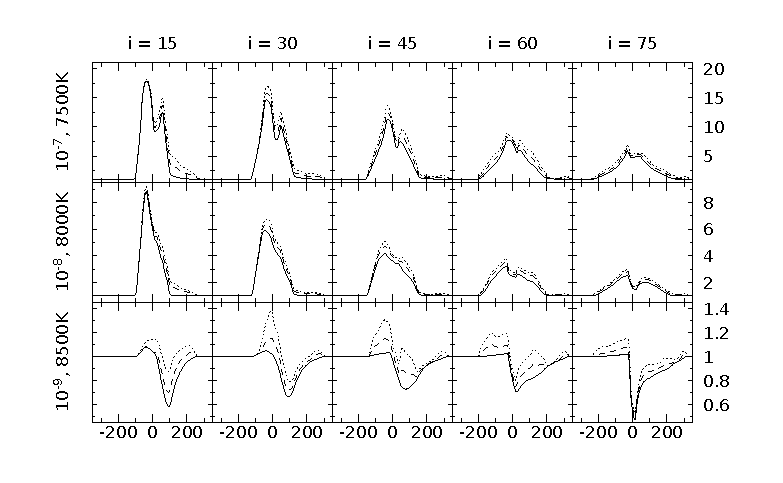
\includegraphics[width=\textwidth]{hot_5_Hb.eps}
\end{figure}
\end{frame}

%\frame[noframenumbering]{Профили линии аш бета показывают в целом туже зависимость, что и профили аш альфа, но в них видно больше деталей, так как нету размытия из-за лоренцевских крыльев. Нагрев снова больше всего влият на малоинтенсивные профили.} 

\begin{frame}
\frametitle{Вращение магнитосферы. Линия H$\beta$}
\begin{figure}[h]
\centering
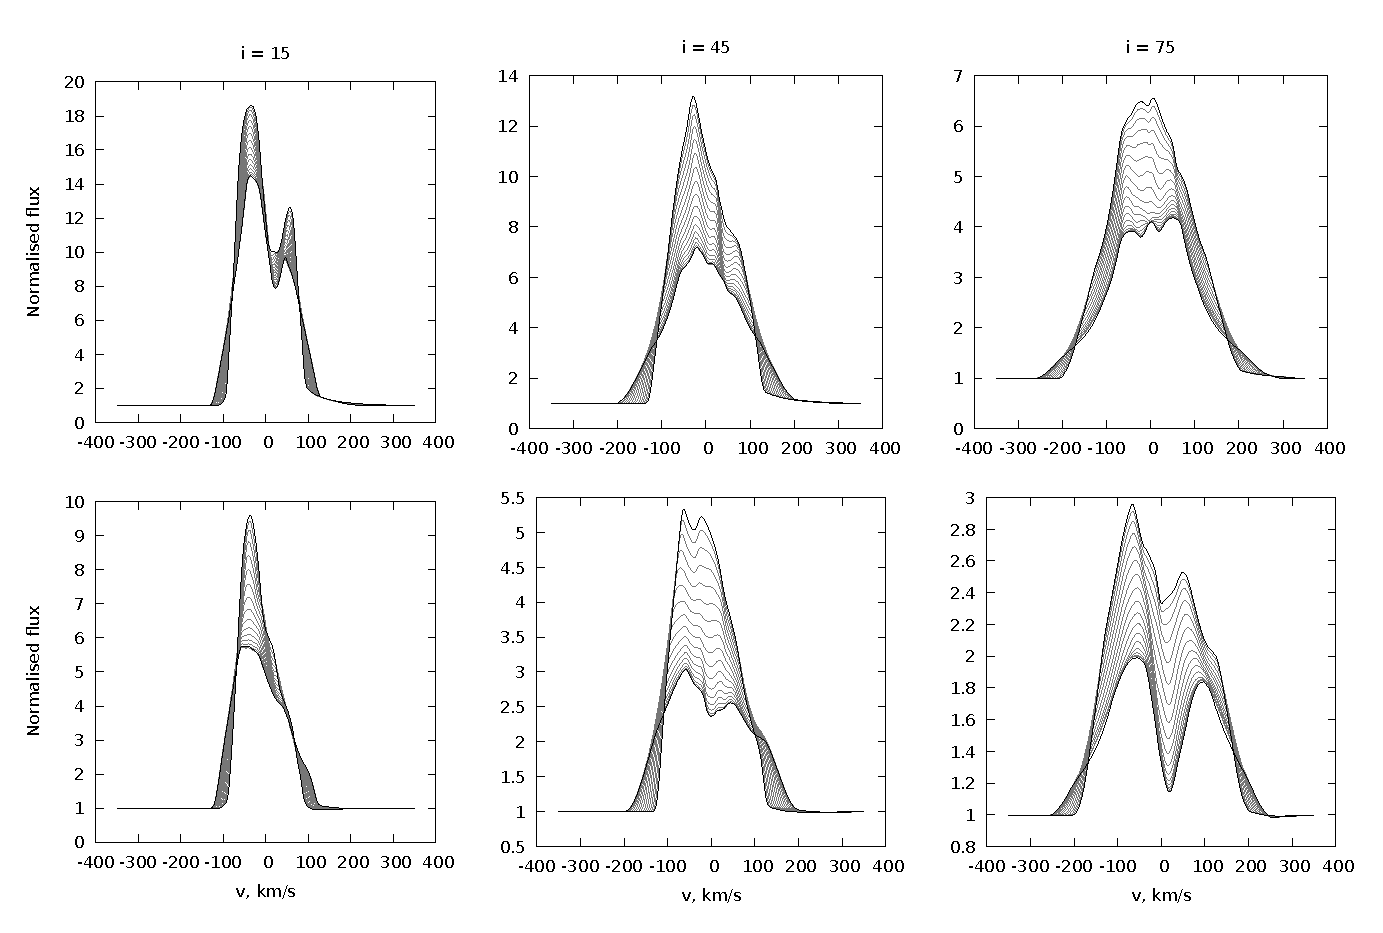
\includegraphics[width=0.9\textwidth]{rot.eps}
\end{figure}
\end{frame}
% \FloatBarrier

%\frame[noframenumbering]{Вращение магнитосферы при угле между осями в 15 градусов. Показаны две модели (-8 8000, -7 7500) с различными углами наклона. Черным выделены крайние фазы ноль и 180 градусов. Переменность выходит качественно похожей на наблюдаемую.} 

\section{Сравнение с наблюдениями}

\begin{frame}
\frametitle{Согласие с наблюдениями}
\begin{figure}[h]
\centering
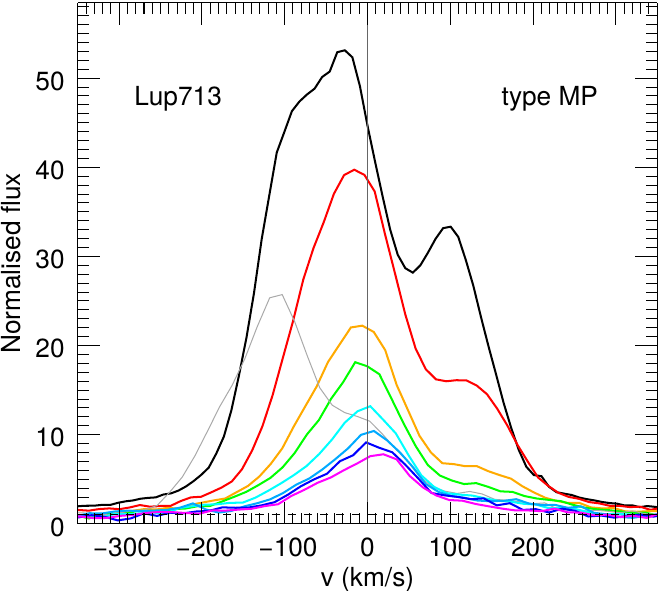
\includegraphics[width=0.45\textwidth]{profiles2.png}
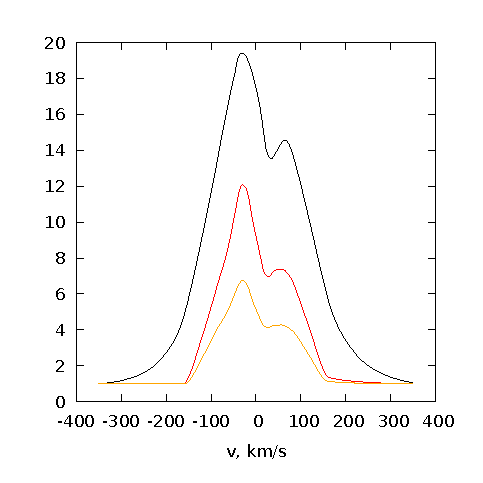
\includegraphics[width=0.4\textwidth]{lookslike45.eps}
\end{figure} 
\end{frame}

%\frame[noframenumbering]{Показаны наблюдаемые профили бальмеровской серии в спектре звезды 713 волка, и также похожие на них теоритечиские профили для темпа аккреции -8.5 и температуры 8000 К. Наблюдается качественное согласие форм профилей линий. }

\section{Заключение}

\begin{frame}
\frametitle{Заключение}
Результаты:
\begin{itemize}
\item Разработан и реализован в виде двух компьютерных программ алгоритм расчета cостояния газа в магнитосфере звезды и образующегося в ней водородного спектра.
\item Исследовано влияние дополнительного нагрева магнитосферы излучением горячего пятна.
\item Исследована вращательная модуляция профилей водородных линий, вызванная наклоном магнитосферы относительно оси вращения звезды.
\end{itemize}
\end{frame}

\begin{frame}
\begin{center}
\Huge Спасибо за внимание!
\end{center}
\end{frame}

% \begin{frame}[noframenumbering]
% \begin{thebibliography}{99}
% % % \bibitem{hartmann94}{\it 
% % % Хартманн и др.} (L. Hartmann, R. Hewett, N. Calvet), Astrophys. J. {\bf 426}, 669 (1994). 

% % % \bibitem{lima10}{\it Лима и др.} (G.H.R.A. Lima, S.H.P. Alencar, N. Calvet \etal ) Astron. Astrophys. {\bf 522}, A104 (2010)

% % % \bibitem{hartmann01}{\it Мацеролли и др.} (J. Muzerolle, N. Calvet, L. Hartmann ) Astrophys. J. {\bf 550}, 944 (2001)

% % % \bibitem{rybicki78}{\it Райбики, Хаммер } (G.B. Rybicki, D.G. Hummer ) Astrophys. J. {\bf 219}, 654 (1978)

% % % \bibitem{grachev75}{\it Грачев С.И., Гринин В.П.}, Астрофизика {\bf 11}, 20 (1975)

% % % \bibitem{katysheva80} Катышева Н.А., Гринин В.П., Изв. КрАО, 1980, 62, 52

% % \bibitem{petrov03} Петров, П.П., Астрофизика, 2003, том 46, No 4, c. 506
% % \bibitem{matt05} Matt, S., Pudritz, R.E., ApJL, 2005, 632, L135
% % \bibitem{muzerolle01} Muzerolle, J., Calvet, N., \etal, ApJ, 2001, 550, 944
% % \bibitem{lima10} Lima, G.H.R.A., Alencar, S.H.P., \etal, A\&A, 2010, 522, A104
% \bibitem{antoniucci17} Antoniucci, S., Nisini, B., \etal, A\&A, 2017, 599, A105
% % \bibitem{tambovtseva14} Tambovtseva, L.V., Grinin, V.P, \etal, A\&A, 2014, 562, A104
% % \bibitem{grinin11} Гринин В.П., Tамбовцева, Л.В., АЖ, 2011, том 88, No 8, с. 766
% \bibitem{hartmann94} Hartmann, L., Hewett, R., \etal, ApJ, 1994, 426, 669
% % \bibitem{bouvier99} Bouvier, J., Chelli A., \etal, A\&A, 1999, 349, 619
% % \bibitem{petrov01} Petrov, P.P., Gahm, G.F., \etal, A\&A, 2001, 369, 993
% \bibitem{dodin18} Dodin, A., MNRAS, 2018, 475, 4367
% % \bibitem{lamzin98} Ламзин, С.А., АЖ, 1998, 47, 498
% \bibitem{grachev75} Грачев, С.И., Гринин, В.П., Астрофизика, 1975, 11, 20 
% \bibitem{rybicki78} Rybicki, G.B., Hummer, D.G., ApJ, 1978, 550, 944
% % \bibitem{katysheva80} Катышева, Н.А., Гринин, В.П., Изв. КрАО, 1980, 62, 52
% % \bibitem{alencar18} Alencar, S.H.P., Teixeira, P.S., \etal, A\&A, 2010, 519, A88 
% % \bibitem{luttermoser92} Luttermoser, D.G., Johnson, H.R., ApJ, 1992, 388, 579
% % \bibitem{humlicek82} Humlicek, J., J. Quant. Spectrosc. Radiat. Transfer, 1982, Vol. 27, No. 4, P. 437 
% % % \bibitem{kenyon95} Kenyon, S.J., Hartmann L., 1995, ApJS, 101, 117
% % % \bibitem{palla99} Palla, F., Stahler, S. W., 1999, ApJ, 525, 772
% % % \bibitem{dullemond07} Dullemond, C.P., et al., 2007, Protostars and Planets V (Tuscon,AZ: Univ. Arizona Press),555
% % % \bibitem{krull99} Johns-Krull, C.M., et al. A.1999, ApJL, 510, L41
% % % \bibitem{gunther13} Gunther, H. M. 2013, AN, 334, 67
% \bibitem{sousa16} Sousa, A.P., Alencar, S.H.P., \etal, A\&A, 2016, 586, A47
% % % \bibitem{cranmer09} Cranmer, S. R.: 2009, ApJ 706, 824
% % % \bibitem{matt07} Matt, S. \& Pudritz, R. E.: 2007, in IAU Symposium, Vol. 243, p. 299
% % % \bibitem{herbst94} Herbst, W. et al. 1994,AJ, 108, 1906
% % % \bibitem{petrov99} Petrov, P.P. et al. 1999, A\& ;A, 341, 553

% \end{thebibliography}
% % \end{document}
% \end{frame}

\begin{frame}[noframenumbering]
\frametitle{Альфвеновский радиус}
\begin{equation}
r_A/R_\star =\frac{B_\star^{4/7}R_\star^{5/7}}{\dot{M}^{2/7}(2GM_\star)^{1/7}}
\end{equation}
\end{frame}

\begin{frame}[noframenumbering]
\frametitle{Движение газа в магнитосфере}
Скорость газа в магнитосфере в сферической системе координат

\begin{align} \label{eq:velvec}
|\vec{v}&|  = v_\text{esc}\sqrt{\left(\frac{R_\star}{r} - \frac{R_\star}{r_\text{m}}\right)} \\
 \vec{v} & = v \hat{r} + u \hat{\theta}/r\\
 v & = -2v_\text{esc}\sqrt{\frac{R_\star}{r}}\frac{\cos^2\theta}{\sqrt{4-3y}}  \\
 u & = -v_\text{esc}\sqrt{\frac{R_\star}{r}}\frac{\cos\theta\sin\theta}{\sqrt{4-3y}} 
\end{align}

\end{frame}

\begin{frame}[noframenumbering]
\frametitle{Оптическая толщина и градиент скорости}
\begin{equation}
\tau_{ik}(\vec{r},\vec{n}) = \frac{\pi e^2 f_{ik}}{m \nu_{ki} |\vec{n}\cdot \vec{\nabla} (\vec{v}\vec{n})|} n_i \left( 1 - \frac{n_k}{n_i}\frac{g_i}{g_k} \right)
\end{equation} 

\begin{align} \label{eq:vecgrad}
\vec{n}\cdot\vec{\nabla}(\vec{v}\vec{n}) & = \frac{\partial v}{\partial r}\cos^2(\alpha) + \frac{1}{r}\frac{\partial v}{\partial \theta}\cos(\alpha)\sin(\alpha)\cos(\beta) + \frac{v}{r}\sin^2(\alpha) + \nonumber \\
& + \frac{\partial u}{\partial r} \cos(\alpha)\sin(\alpha)\cos(\beta) + \frac{1}{r}\frac{\partial u}{\partial \theta} \sin^2(\alpha)\cos^2(\beta) - \nonumber \\
& - \frac{u}{r}\left(\cos(\alpha)\sin(\alpha)\cos(\beta) - \cot\theta\sin^2(\alpha)\sin^2(\beta)\right)
\end{align}

В случае радиального движения
\[
\vec{n}\cdot \vec{\nabla}(\vec{v}\vec{n}) = \frac{\partial v}{\partial r}\cos^2(\alpha) + \frac{v}{r}\sin^2(\alpha) 
\]

\end{frame}

\begin{frame}[noframenumbering]
\frametitle{Градиент скорости в магнитосфере}
\begin{figure}
\centering
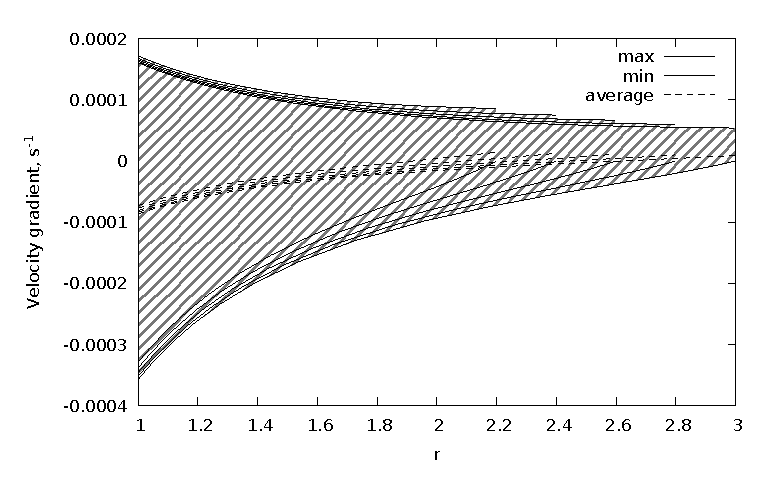
\includegraphics[width=0.9\textwidth]{grad}
\end{figure}
\end{frame}

\begin{frame}[noframenumbering]
\frametitle{Ориeнтация магнитосферы}
\begin{figure}
\centering
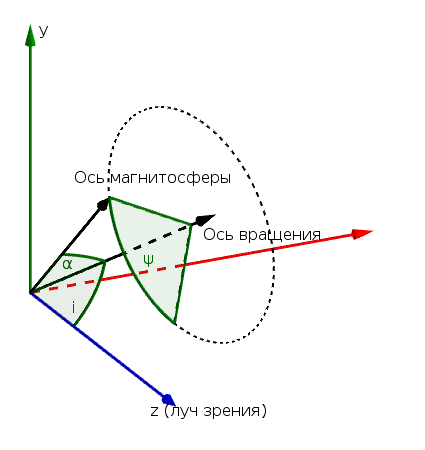
\includegraphics[width=0.5\textwidth]{axis.png}
\end{figure}
\end{frame}

\begin{frame}[noframenumbering]
\frametitle{Интенсивность в линии}
\begin{equation} \label{eq:profmain}
I_{\nu} = \int \limits_{S} I_{xy}(\nu) dS
\end{equation}
\begin{equation}
I_{xy}(\nu) = \int \limits_{z_0}^{z_k} S_{ul}(z)k_{lu}(\nu,z)e^{-\tau(\nu,z)}dz 
\end{equation}
\begin{equation} \label{eq:profdepth}
\tau(\nu,z) = \int \limits_z^{z_k} k_{lu}(\nu,z')dz' 
\end{equation}
\begin{equation} \label{eq:profsource}
S_{ul}(z) = \frac{2h\nu_0^3}{c^2}\left(\frac{n_l}{n_u} \frac{g_u}{g_l} - 1 \right)^{-1} 
\end{equation}
\begin{equation} \label{eq:profabsorb}
k_{lu}(\nu,z) = 0.02654f_{lu}\alpha(\nu, z)n_l\left(1 - \frac{g_l}{g_u}\frac{n_u}{n_l}\right) 
\end{equation}

\end{frame}

\begin{frame}[noframenumbering]
\frametitle{Расчет профиля линии}
\begin{equation} \label{eq:profcont}
I_c = \frac{2h\nu^3}{c^2}\frac{1}{\exp\left(\frac{h\nu}{k_bT_\star}\right)-1} 
\end{equation}

\begin{equation} \label{eq:profnorm}
r_{\nu} = \frac{I_\nu + I_{\tau}(\nu)}{I_c \pi R_\star^2} 
\end{equation}

\begin{equation} \label{eq:absorbprof}
I_{\tau}(\nu) = \int \limits_{S_\star} I_c e^{-\tau} dS 
\end{equation}
\end{frame}

\begin{frame}[noframenumbering]
\frametitle{Сетка в магнитосфере}
\begin{figure}
\centering
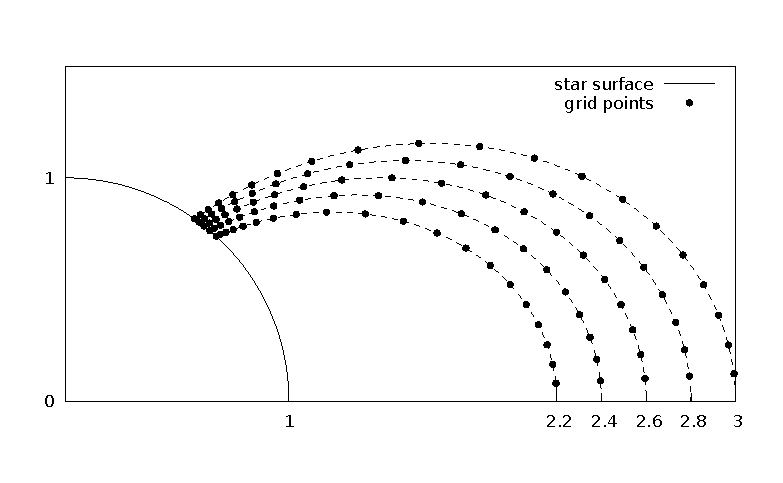
\includegraphics[width=0.9\textwidth]{grid}
\end{figure}
\end{frame}

\begin{frame}[noframenumbering]
\frametitle{Профили водородных линий. H$\gamma$}
\begin{figure}[h]
\centering
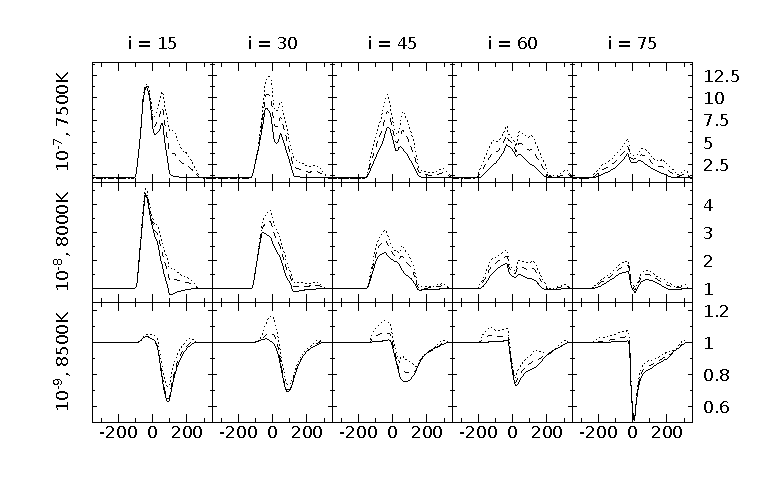
\includegraphics[width=\textwidth]{hot_5_Hg.eps}
\end{figure}
\end{frame}

\begin{frame}[noframenumbering]
\frametitle{Профили водородных линий. Br$\gamma$}
\begin{figure}[h]
\centering
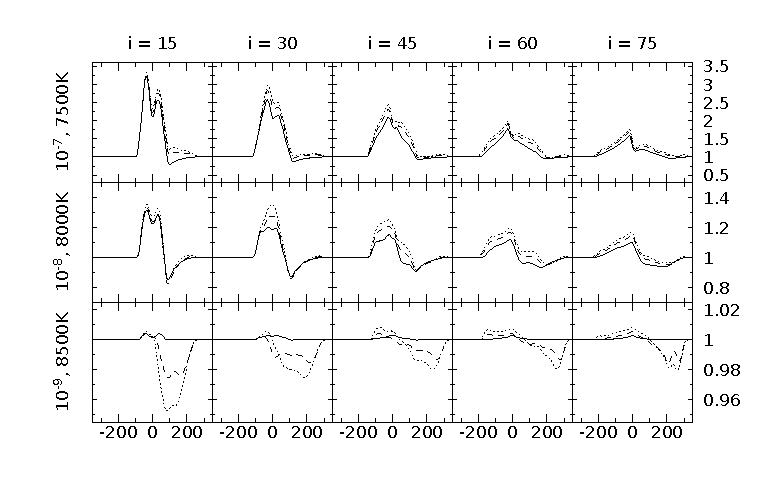
\includegraphics[width=\textwidth]{hot_5_Brg.eps}
\end{figure}
\end{frame}





% Основным результатом данной работы является программная реализация алгоритма, позволяющего моделировать профили магнитосферных линий в спектрах молодых звезд. 
% %Эту модель можно использовать вместе с существующими моделями ветров для определения параметров магнитосферы, таких как темп аккреции и температура в ней. 
% Полученные профили водородных линий похожи на теоретические профили из работ Хартманна \cite{hartmann94} и Мацеролле \cite{muzerolle01}. Полного совпадения ожидать нельзя, так как модели не совсем идентичны. Сравнение с наблюдениями показало, что теоретические профили хорошо воспроизводят все основные детали наблюдаемых, в спектрах, с преобладающим вкладом излучения магнитосферы. 

% Также мы продемонстрировали возможность моделировать наблюдаемую переменность линий вращением магнитосферы, ось которой наклонена относительно оси вращения звезды.

% \begin{thebibliography}{99}
% % \bibitem{hartmann94}{\it 
% % Хартманн и др.} (L. Hartmann, R. Hewett, N. Calvet), Astrophys. J. {\bf 426}, 669 (1994). 

% % \bibitem{lima10}{\it Лима и др.} (G.H.R.A. Lima, S.H.P. Alencar, N. Calvet \etal ) Astron. Astrophys. {\bf 522}, A104 (2010)

% % \bibitem{hartmann01}{\it Мацеролли и др.} (J. Muzerolle, N. Calvet, L. Hartmann ) Astrophys. J. {\bf 550}, 944 (2001)

% % \bibitem{rybicki78}{\it Райбики, Хаммер } (G.B. Rybicki, D.G. Hummer ) Astrophys. J. {\bf 219}, 654 (1978)

% % \bibitem{grachev75}{\it Грачев С.И., Гринин В.П.}, Астрофизика {\bf 11}, 20 (1975)

% % \bibitem{katysheva80} Катышева Н.А., Гринин В.П., Изв. КрАО, 1980, 62, 52

% \bibitem{petrov03} Петров, П.П., Астрофизика, 2003, том 46, No 4, c. 506
% \bibitem{hartmann94} Hartmann, L., Hewett, R., \etal, ApJ, 1994, 426, 669
% \bibitem{matt05} Matt, S., Pudritz, R.E., ApJL, 2005, 632, L135
% \bibitem{muzerolle01} Muzerolle, J., Calvet, N., \etal, ApJ, 2001, 550, 944
% \bibitem{lima10} Lima, G.H.R.A., Alencar, S.H.P., \etal, A\&A, 2010, 522, A104
% \bibitem{grachev75} Грачев, С.И., Гринин, В.П., Астрофизика, 1975, 11, 20 
% \bibitem{rybicki78} Rybicki, G.B., Hummer, D.G., ApJ, 2001, 550, 944
% \bibitem{tambovtseva14} Tambovtseva, L.V., Grinin, V.P, \etal, A\&A, 2014, 562, A104
% \bibitem{grinin11} Гринин В.П., Tамбовцева, Л.В., АЖ, 2011, том 88, No 8, с. 766
% \bibitem{antoniucci17} Antoniucci, S., Nisini, B., \etal, A\&A, 2017, 599, A105
% \bibitem{bouvier99} Bouvier, J., Chelli A., \etal, A\&A, 1999, 349, 619
% \bibitem{petrov01} Petrov, P.P., Gahm, G.F., \etal, A\&A, 2001, 369, 993
% \bibitem{dodin18} Dodin, A., MNRAS, 2018, 475, 4367
% \bibitem{lamzin98} Ламзин, С.А., АЖ, 1998, 47, 498
% \bibitem{katysheva80} Катышева, Н.А., Гринин, В.П., Изв. КрАО, 1980, 62, 52
% \bibitem{alencar18} Alencar, S.H.P., Teixeira, P.S., \etal, A\&A, 2010, 519, A88 
% \bibitem{luttermoser92} Luttermoser, D.G., Johnson, H.R., ApJ, 1992, 388, 579
% \bibitem{humlicek82} Humlicek, J., J. Quant. Spectrosc. Radiat. Transfer, 1982, Vol. 27, No. 4, P. 437 
% % \bibitem{kenyon95} Kenyon, S.J., Hartmann L., 1995, ApJS, 101, 117
% % \bibitem{palla99} Palla, F., Stahler, S. W., 1999, ApJ, 525, 772
% % \bibitem{dullemond07} Dullemond, C.P., et al., 2007, Protostars and Planets V (Tuscon,AZ: Univ. Arizona Press),555
% % \bibitem{krull99} Johns-Krull, C.M., et al. A.1999, ApJL, 510, L41
% % \bibitem{gunther13} Gunther, H. M. 2013, AN, 334, 67
% \bibitem{sousa16} Sousa, A.P., Alencar, S.H.P., \etal, A\&A, 2016, 586, A47
% % \bibitem{cranmer09} Cranmer, S. R.: 2009, ApJ 706, 824
% % \bibitem{matt07} Matt, S. \& Pudritz, R. E.: 2007, in IAU Symposium, Vol. 243, p. 299
% % \bibitem{herbst94} Herbst, W. et al. 1994,AJ, 108, 1906
% % \bibitem{petrov99} Petrov, P.P. et al. 1999, A\& ;A, 341, 553

% \end{thebibliography}
\end{document}